% page 1 2
\begin{center}
\raisebox{-18mm}{
\includegraphics[scale=0.33]{xjtu/xjtu1}} \hskip 44mm
\begin{tabular}{|C{22mm}|C{34mm}|}
	\hline
	\parbox[c][8.2mm][c]{0pt}{}{\kai\bf\xiaosi 学\hspace*{7mm} 院} & {\kai\bf\xiaosi\institution} \\
	\hline
	\parbox[c][8.2mm][c]{0pt}{}{\kai\bf\xiaosi 编\hspace*{7mm} 号} & {\kai\bf\xiaosi\numberID} \\
	\hline
	\end{tabular}\\
\vspace{8mm}
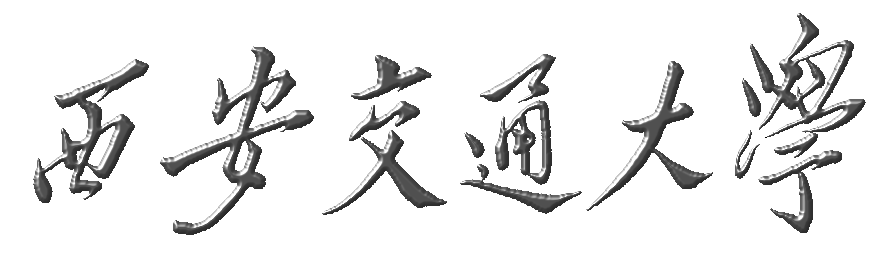
\includegraphics[scale=0.31]{xjtu/xjtu2}
\vspace{3mm}

{\song\xiaochu\bf
博士研究生\\[6mm]
中期进展报告}
\vspace{35mm}

{\large\sanhao%\renewcommand{\arraystretch}{0.9}
\renewcommand\arraystretch{1.32}
\begin{tabular}{lc}
\makebox[26mm][s]{\kai\bf\xiaosan 学    号:}   & \underline{\makebox[16em][c]{\xiaosan\kai\cardID}}\\
\makebox[26mm][s]{\kai\bf\xiaosan 研 究 生:}  & \underline{\makebox[16em][c]{ \xiaosan\kai\namestudent}}\\
\makebox[26mm][s]{\kai\bf\xiaosan 导   师:}   & \underline{\makebox[16em][c]{\xiaosan\kai\namesupervisor}}\\
\makebox[26mm][s]{\kai\bf\xiaosan 论 文 题 目:}& \underline{\makebox[16em][c]{\xiaosan\kai\thestitlelineone}}\\
                                               & \underline{\makebox[16em][c]{\xiaosan\kai\thestitlelinetwo}}\\
%                                           & \underline{\makebox[16em][c]{\xiaosan\kai\thestitlelinethree}}\\
\makebox[26mm][s]{\kai\bf\xiaosan 学    科:}   & \underline{\makebox[16em][c]{\xiaosan\kai\discipline}}\\
\makebox[26mm][s]{\kai\bf\xiaosan 填 写 时 间:}& \underline{\makebox[16em][c]{ \myyear ~年 \mymonth ~月 \myday ~日}}
\end{tabular}
}\\
\vspace{10mm}
{\kai\xiaosan 西安交通大学研究生院制}
\end{center}
\thispagestyle{empty}


\newpage
\vspace*{-7mm}
\begin{center}
\hei\xiaosan 填  写  说  明 \\
\vspace{15mm}
\begin{minipage}{13.6cm}
{%\linespread{1.5}
\song\sihao
\hspace{1.6em} 一、博士研究生中期进展报告必须采用 A4 纸双面打印,左侧装订成册,各栏空格不够时,请自行加页。格式可在研究生院主页下载。\vspace*{2mm}
\par \linespread{1.5} \hspace{1.6em} 二、中期进展报告正文部分字数为 8000-10000 字。\vspace*{2mm}
\par \linespread{1.5} \hspace{1.6em} 三、博士研究生中期进展报告通过后,\vspace*{2mm} 本报告由学院存档,并作为必修环节,登入成绩。
}
\end{minipage}
\end{center}

\thispagestyle{empty}
